% Postavke dokumenta i osnovne informacije

\documentclass[a4paper,12pt]{foi}

\renewcommand{\brojAutora}{1} % Broj autora rada (max. 6)

\renewcommand{\naslov}{Praćenje aktivnosti na društvenim mrežama pomoću reaktivnih agenata} % Naslov rada

\renewcommand{\mentor}{Doc. dr. sc. Markus Schatten} % Ime i prezime mentora

\renewcommand{\autorA}{Nikola Majcen} % Ime i prezime autora
\renewcommand{\brIndeksaA}{44445/15-R} % Broj indeksa autora

\renewcommand{\vrstaRada}{Seminarski rad}
\lfoot{Kolegij: Višeagentni sustavi}

\usepackage{graphicx}
\usepackage[export]{adjustbox}
\graphicspath{ {img/} }

% Sadržaj

\begin{document}

\maketitle

\tableofcontents

\thispagestyle{empty}

\setcounter{page}{0}

\onehalfspacing

% Uvod

\chapter{Uvod}

Tema ovog seminarskog rada je praćenje aktivnosti na društvenim mrežama pomoću reaktivnih agenata, odnosno izrada jednostavne aplikacije gdje se pomoću agenata mogu pratiti objave na društvenim mrežama u realnom vremenu.

Seminarski rad uključuje teorijsku obradu agenata, ali praktični prikaz i implementaciju rješenja koje je vezano za praćenje aktivnosti na društvenim mrežama Twitter i Facebook. Praćenje na društvenim mrežama uključuje praćenje statusa i/ili hashtag-ova. Rad je podjeljen na cjeline i to:

\begin{itemize}
\item{Opis zadatka}
\item{Implementacija rješenja}
\item{Demonstracija rješenja}
\end{itemize}


% Opis zadatka
\chapter{Opis zadatka}

Tema ovog seminarskog rada jest izrada aplikacije koja korisniku omogućuje da pretražuje određene društvene mreže preko hashtag-ova ili statusa, na način da se na iste pretplati te obrada literature vezane za reaktivne agente koji se koriste u samoj aplikaciji.

\section{Koncept zadatka}
Da bi korisnik mogao pretraživati određene društvene mreže, za početak je potrebno pretpostaviti koji će biti elementi pretrage i kako će se moći podaci pratiti. 

U ovom zadatku će se koristiti društvene mreže Facebook i Twitter, gdje će se kod svake od njih pratiti određena aktivnost korisnika. Zbog određenih mjera privatnosti, nije bilo moguće izvesti iste funkcionalnosti za svaku od društvenih mreža, pa je shodno tome omogućeno sljedeće; za društvenu mrežu Facebook omogućeno je:

\begin{itemize}
\item{Praćenje statusa korisnika čiji su profili javni}
\end{itemize}
dok je za društvenu mrežu Twitter omogućeno sljedeće:
\begin{itemize}
\item{Praćenje statusa (tweet) svih korisnika (korisnički profil ne mora biti javan)}
\item{Praćenje statusa (tweet) koji sadrže određeni hashtag}
\end{itemize}

Pretplata na promjenu statusa ili praćenje statusa sa određenim hashtag-om odvija se na način da korisnik definira vrijeme u sekundama u kojim će intervalima i kolko dugo pratiti promjene na određenoj društvenoj mreži. Detaljnije informacije o implementaciji zadatka i potrebnim dodatnih podacima za spajanje na određene društvene mreže nalaze se u sljedećem poglavlju.

Za implementaciju rješenja ovog zadatka koristio sam višeagentni sustav koji se sastoji od dva, odnosno tri reaktivna agenta. Dva reaktivna agenta omogućuju pretraživanje i praćenje promjena na društvenim mrežama, a skupljene podatke šalju trećem agentu koji dohvaća sve promjene svih agenata. Za svaku društvenu mrežu definiran je posebni agent koji koristi specifične načine dohvata podataka za svaku od društvenih mreža. Nakon što određeni agent za dohvaćanje podataka s društvene mreže završi s radom, treći agent (koji sakuplja podatke) šalje izvještaj u obliku svih sakupljenih podataka koje mu je taj agent poslao. Na taj način završava praćenje i izvještavanje za tog agenta, dok svi ostali nastavljaju s radom.

\section{Višeagentni sustavi i njihova primjena u društvenim mrežama}



\citep{ArandaPalanca2012} \citep{JonkerTreur2002} \citep{Lerman2008}


% Implementacija rješenja

\chapter{Implementacija rješenja}

U ovom poglavlju prikazat ću implementaciju rješenja za praćenje na društvenim mrežama. Za implementaciju je korišten programski jezik Python verzije 2.7. Kao biblioteka koja omogućuje rad s agentima korišten je SPADE.

Za početak rada, potrebno je u izvornom direktoriju otvoriti datoteku \textit{config.json} te unutar nje definirati naziv i lozinku agenta izvjestitelja. Zadano ime agenta je \textit{reporter@127.0.0.1}, dok je lozinka \textit{secret}.

Uz tu datoteku, postoji i datoteka \textit{credentials-sample.json}, koja predstavlja podatke koji su potrebni da bi se aplikacija mogla povezati sa određenom društvenom mrežom. Detaljnije informacije za unos podataka za svaku od društvenih mreža bit će prikazane u zasebnom poglavlju za svakog agenta posebno, ali prije korištenja potrebno je istu preimenovati u \textit{credentials.json}.

\section{Implementacija Facebook agenta}

Prije detaljnog objašnjavanja Facebook agenta, potrebno je prvo definirati potrebne podatke kako bi se aplikacija mogla povezati sa Facebook servisima. 
Za to je potrebno otvoriti datoteku \textit{credentials.json} te unutar objekta \texttt{facebook} za ključ \texttt{access\_token} unijeti vrijednost tokena koja se dobije kada se kreira nova aplikacija unutar Facebook-ovog sučelja za razvijatelje aplikacija. Bez vrijednosti \texttt{access\_token}-a nije moguće koristiti Facebook agenta.

Prikaz implementacije podijeljen je na tri dijela, a prikazuju sljedeće:

\begin{itemize}
\item{implementaciju modela,}
\item{implementaciju API-a}
\item{implementaciju reaktivnog agenta}
\end{itemize}

\subsection{Prikaz implementacije modela}

Kako bi se dohvatili podaci za spajanje na Facebook-ov servis, kreiran je model \textit{FacebookCredentials}, a sadrži sljedeće:

\definecolor{lbcolor}{rgb}{0.9,0.9,0.9}
\lstset{commentstyle=\textit,language=python}
\lstset{backgroundcolor=\color{lbcolor},rulecolor=}
\lstinputlisting{/Users/nikolamajcen/Development/Python/social-notifier/social/facebook/facebook_credentials.py}

Model sadrži dvije metode; \texttt{get\_credentials()} za dohvat podataka za spajanje na servis, te \texttt{\_\_read\_configuration\_file()} koja omogućuje čitanje datoteke u kojem se nalaze podaci za spajanje na servis.

Sljedeći modeli su \textit{FacebookUser} i \textit{FacebookStatus}:

\definecolor{lbcolor}{rgb}{0.9,0.9,0.9}
\lstset{commentstyle=\textit,language=python}
\lstset{backgroundcolor=\color{lbcolor},rulecolor=}
\lstinputlisting{/Users/nikolamajcen/Development/Python/social-notifier/social/facebook/facebook_models.py}

Klasa \textit{FacebookUser} definira osnovne informacije o korisniku, kao što je njegov id, korisničko ime, ime i prezime te lokacija. Podaci se dobivaju na način da se preko konstruktora prislijedi objekt koji sadrži navedene podatke te se oni otpakiraju na način da se proslijedi ključ, a bit će vraćena vrijednost za navedeni ključ. Klasa \textit{FacebookStatus} definira osnovne informacije o statusu, a sadrži ime i prezime korisnika koji je objavio status, korisničko ime, tip statusa, vrijeme objave, te ovisno o tome da li se radi o tekstualnom statusu ili slici poruku odnosno poveznicu. Način dobivanja podataka je identičan kao i za klasu \textit{FacebookUser}.

\subsection{Prikaz implementacije API-a}

Sljedeće što sam kreirao je Facebook API koji zapravo definira pozive metoda koje se spajaju na Facebook-ov službeni API te na temelju tih poziva se dobivaju određeni podaci koje korisnik traži.

\definecolor{lbcolor}{rgb}{0.9,0.9,0.9}
\lstset{commentstyle=\textit,language=python}
\lstset{backgroundcolor=\color{lbcolor},rulecolor=}
\lstinputlisting{/Users/nikolamajcen/Development/Python/social-notifier/social/facebook/facebook_api.py}

Klasa \textit{FacebookAPI} definira samo jedan poziv, a to je dohvaćanje novih statusa. Taj poziv izvršava se preko metode \texttt{search\_posts(username)}. Ova metoda na temelju korisničkog id-a traži nove statuse ili slike korisnika, te iste dohvaća i vraća kao rezultat. Prethodno navedena metoda mora obavezno imati id korisničkog računa potrebnog za dohvaćanje podataka, a kako bi se isti dobio, potrebno je pomoću metode \texttt{\_\_fetch\_user\_details(username)} dohvatiti korisnikov id.

Svi pozivi dohvaćanja podataka vrše se preko Facebook-ovog sustava GraphAPI.

\subsection{Prikaz implementacije reaktivnog agenta}

Ovdje ću prikazati konačnu implementaciju agenta koji na Facebook društvenoj mreži dohvaća promjene u smislu novih statusa koji uključuju tekst ili sliku/e.

\definecolor{lbcolor}{rgb}{0.9,0.9,0.9}
\lstset{commentstyle=\textit,language=python}
\lstset{backgroundcolor=\color{lbcolor},rulecolor=}
\lstinputlisting{/Users/nikolamajcen/Development/Python/social-notifier/agents/facebook_agent.py}

Agent ima dvije podklase koje definiraju ponašanje agenta, a to su \textit{FetchBehaviour} i \textit{ReportDeliveryBehaviour}.

\texttt{FetchBehaviour} je ponašanje koje je definirano kao \texttt{PeriodicBehaviour} a ono funkcionira na način da u određenim vremenskim intervalima pokreće metodu \texttt{\_onTick()}. Vrijeme između dva pokretanja navedene metode definira se putem konstruktora klase \texttt{PeriodicBehaviour}. 

Sastoji se od metoda koje su definirane od strane nadklase \texttt{PeriodicBehaviour} gdje se kod metode pokretanja \texttt{onStart()} šalje poruka registracije agentu izvjestitelju o Facebook agentu pomoću metode \texttt{\_\_send\_registration\_message()}. Na taj način agent izvjestitelj vodi evidenciju o prijavljenom agentu i njegovim podacima. U svakom periodu provjerava se da li je broj perioda koje je korisnik definirao iskorišten. Ukoliko jest, onda se prelazi iz metode \texttt{\_onTick()} na samo jedno izvršavanje metode \texttt{onEnd()} gdje se agentu izvjestitelju šalje poruka da agent želi dobiti izvješće i to pomoću metode \texttt{\_\_send\_report\_message()}. U suprotnosti, kada je broj perioda veći od 0, šalje se zahtjev za dohvaćanjem podataka sa Facebook servisa te se provjerava što promijenilo od zadnje provjere. To je omogućeno pomoću metode \texttt{fetch\_data()}. Nakon dohvaćanja podataka, ukoliko je bilo kakve promjene, dohvaćeni podaci se šalju agentu izvjestitelju pomoću metode \texttt{\_\_send\_status\_message()} te se tamo spremaju za daljnje korištenje.

\texttt{ReportDeliveryBehaviour} je ponašanje koje je definirano kao \texttt{EventBehaviour} što predstavlja ponašanje koje je kreirano na način da se okida na neki događaj. Isto tako, potrebno je napomenuti da ovo ponašanje nije instancirano niti pokrenuto tako dugo dok ga ne okine određen događaj.

Sastoji se od metode \texttt{\_process()} koja je definirana nadklasom \texttt{EventBehaviour}, a radi na način da očekuje poruku od agenta izvjestitelja. Kada ju dobije ispiše njen sadržaj na ekran i završi s radom agenta.

Konačno, sam agent \texttt{FacebookAgent} nasljeđuje klasu \texttt{Agent} te se time definiraju konstruktor i metoda \texttt{\_setup()}. Konstruktor je u ovom slučaju definiran drugačije od zadanog, pa je potrebno ručno pozvati konstuktor i proslijediti potrebne podatke. Podaci koje je potrebno proslijediti jesu korisničko ime i lozinka agenta, a to se generira pomoću metode \texttt{\_\_generate\_agent\_credentails()}. Ostali podaci koji su proslijeđeni kroz konstruktor su tražena riječ, vrijeme trajanja periode i broj perioda.

Da bi radilo slanje poruka između agenata, u metodi \texttt{\_setup()} definirana su dva ponašanja,  s time da je bilo potrebno za ponašanje \texttt{ReportDeliveryBehavior} definirati i predložak sa definiranom ontologijom što je u ovom slučaju \texttt{delivery\_template}.

\section{Implementacija Twitter agenta}

U ovom potpoglavlju prikazat ću način na koji sam implementirao Twitter agenta. Prije prikaza same implementacije, potrebno je naglasiti, kao i kod Facebook agenta, da je važno da se unutar datoteke \textit{credentials.json} unesu potrebne vrijednosti za \texttt{api\_key}, \texttt{api\_key\_secret}, \texttt{access\_token} i \texttt{access\_token\_secret}. Navedene podatke je moguće dobiti nakon što se kreira nova aplikacija unutar Twitter aplikacije u dijelu za razvijatelje aplikacija.

\subsection{Prikaz implementacije modela}

Za dobivanje podataka potrebnih za spajanje na Twitter-ov servis, koristio sam sljedeću klasu \textit{TwitterCredentials}. Pomoću metode \texttt{\_\_read\_configuration()} dohvaća se datoteka unutar koje se nalaze podaci o spajanju na Twitter servis, dok se pomoću metode \texttt{get\_credentials()} dohvaćaju navedeni podaci iz datoteke te vraćaju kao n-torka.

\definecolor{lbcolor}{rgb}{0.9,0.9,0.9}
\lstset{commentstyle=\textit,language=python}
\lstset{backgroundcolor=\color{lbcolor},rulecolor=}
\lstinputlisting{/Users/nikolamajcen/Development/Python/social-notifier/social/twitter/twitter_credentials.py}

Sljedeća klasa koja predstavlja model je \textit{TwitterPost}. Ova klasa sadrži osnovne podatke o statusu odnosno tweet-u, a to su redom; vrijeme objave, id posljednje objave, tekst statusa, korisničko ime, ime i prezime korisnika te lokacija.

\definecolor{lbcolor}{rgb}{0.9,0.9,0.9}
\lstset{commentstyle=\textit,language=python}
\lstset{backgroundcolor=\color{lbcolor},rulecolor=}
\lstinputlisting{/Users/nikolamajcen/Development/Python/social-notifier/social/twitter/twitter_models.py}

\subsection{Prikaz implementacije API-a}

Sljedeće što je potrebno da bi Twitter agent radio i dohvaćao podatke je API koji definira metode pomoću kojih je moguće spajanje na Twitter servis. Na taj način se dobivaju podaci ovisno da li se radi o dohvaćanju statusa korisnika ili novih statusa na temelju hashtag-a.

\definecolor{lbcolor}{rgb}{0.9,0.9,0.9}
\lstset{commentstyle=\textit,language=python}
\lstset{backgroundcolor=\color{lbcolor},rulecolor=}
\lstinputlisting{/Users/nikolamajcen/Development/Python/social-notifier/social/twitter/twitter_api.py}

Definirane su dvije osnovne metode pomoću kojih se dohvaćaju podaci preko API-a. To su metode \texttt{search\_hashtag(hashtag, since\_id} i \texttt{search\_tweets(username, since\_id)}.

Metoda \texttt{search\_hashtag(hashtag, since\_id)} traži sve statuse koji sadrže navedeni hashtag, a nastali su nakon prethodnog traženja od strane korisnika što u ovom slučaju predstavlja parameter \texttt{since\_id}. Metoda \texttt{search\_tweets(username, since\_id(} traži nove statuse od određenog korisnika koji su nastali nakon zadnje pretrage. Obje metode nakon pozivanja vraćaju statuse koji su dohvaćeni u navedenom vremenu.

\subsection{Prikaz implementacije reaktivnog agenta}

Ovdje ću prikazati konačnu implementaciju agenta koji na Twitter društvenoj mreži dohvaća promjene u smislu novih statusa od stane korisnika ili novih statusa koji sadrže definirani hashtag.

\definecolor{lbcolor}{rgb}{0.9,0.9,0.9}
\lstset{commentstyle=\textit,language=python}
\lstset{backgroundcolor=\color{lbcolor},rulecolor=}
\lstinputlisting{/Users/nikolamajcen/Development/Python/social-notifier/agents/twitter_agent.py}

Agent ima dvije podklase koje definiraju ponašanje agenta, a to su \textit{FetchBehaviour} i \textit{ReportDeliveryBehaviour}.

\texttt{FetchBehaviour} je ponašanje koje je definirano kao \texttt{PeriodicBehaviour}. Sastoji se od metoda koje su definirane od strane nadklase \texttt{PeriodicBehaviour} gdje se kod pokretanja kod metode \texttt{onStart()} šalje poruka registracije agentu izvjestitelju o Twitter agentu pomoću metode \texttt{\_\_send\_registration\_message()}  kako bi agent izvjestitelj mogao voditi evidenciju o njemu i njegovim podacima. U svakom periodu u metodi \texttt{\_onTick()} provjerava se da li je broj perioda koje je korisnik definirao iskorišten. Ukoliko jest, onda se prelazi iz metode \texttt{\_onTick()} na samo jedno izvršavanje metode \texttt{onEnd()} gdje se agentu izvjestitelju šalje poruka da agent želi dobiti izvješće i to pomoću metode \texttt{\_\_send\_report\_message()}. U suprotnosti se šalje zahtjev za provjerom da li se na Twitter servisu što promijenilo od zadnje provjere. Ovdje je važno spomenuti da se na temelju korisničkog unosa odnosno definiranja pretrage šalje različiti zahtjev, tj. poziva se različita metoda. Metoda koja se koristi za dohvaćanje novih podataka je \texttt{fetch\_data()} te ona poziva \texttt{self.twitter\_api.search\_tweets(username, since\_id)} ako je korisnik kao vrstu pretrage odabrao \textit{hashtag}, dok se u slučaju vrste pretrage \textit{tweet} poziva metoda \texttt{self.twitter\_api.search\_hashtags(hashtag, since\_id)}. Nakon što se podaci dohvate, isti se šalju agentu izvjestitelju.

\texttt{ReportDeliveryBehaviour} je ponašanje koje je definirano kao \texttt{EventBehaviour}. Sastoji se od samo jedne metode koja je definirana nadklasom \texttt{EventBehaviour}, a radi na način da očekuje poruku od agenta izvjestitelja, a kada ju dobije ju ispiše na ekran i završi s radom agenta.

Konačno, sam agent \texttt{TwitterAgent} nasljeđuje klasu \texttt{Agent} te se time definiraju konstruktor i metoda \texttt{\_setup()}. Konstruktor je u ovom slučaju definiran drugačije od zadanog, pa je potrebno ručno pozvati konstuktor i proslijediti potrebne podatke. Podaci koje je potrebno proslijediti jesu korisničko ime i lozinka agenta, a to se generira pomoću metode \texttt{\_\_generate\_agent\_credentails()}.

Radi slanje poruka između agenata, u metodi \texttt{\_setup()} definirana su dva ponašanja isto kao i kod Facebook agenta kako bi se poruke procesuirale na odgovarajući način.

\section{Implementacija agenta za izvještaje}

Važna stavka ovog rješenja je agent izvjestitelj. Ovaj agent zadužen je za prihvaćanje svih informacija koje dobije od agenata koji dohvaćaju podatke s društvenih mreža te na kraju rada svakog pojedinog agenta vraća istome konačan skup njegovih podataka.

Da bi agent mogao komunicirati s agentima koji dohvaćaju podatke s društvenih mreža (Facebook, Twitter), definirana je klasa koja predstavlja model poruke pomoću koje se šalju konačni rezultati odnosno izvještaj za određenog agenta.
Klasa \textit{ReportMessage} sadrži informacije o poruci kao što je vrsta mreže koja predstavlja o kojem se agentu radi (Facebook ili Twitter), vrsti poruke koja predstavlja da li se radi o statusu ili slici, traženoj riječi, korisničkom imenu, imenu i prezimenu korisnika, datumu i sadržaju statusa.
Također, pošto se radi o JSON tipu poruke koja služi za komunikaciju između agenata, potrebno je moći pročitati sadržaj, a za to služi metoda \texttt{load\_json(data)}. Uz to, definirana je metoda za ispis rezultata kako bi on bio definiran na razini modela, a naziv metode je \texttt{print\_message()}.

\definecolor{lbcolor}{rgb}{0.9,0.9,0.9}
\lstset{commentstyle=\textit,language=python}
\lstset{backgroundcolor=\color{lbcolor},rulecolor=}
\lstinputlisting{/Users/nikolamajcen/Development/Python/social-notifier/social/shared/report_message.py}

Agent je implementiran u klasi \textit{ReportAgent} te ima tri podklase koje definiraju ponašanje agenta, a to su \textit{RegisterBehaviour}, \textit{NotifyBehaviour} i \textit{ReportBehaviour}.

Sva tri ponašanja definirana su kao \texttt{EventBehaviour}, a nešto više o toj vrsti ponašanja rečeno je u ranijim poglavljima.

\texttt{RegisterBehaviour} se sastoji od metode \texttt{\_process()} koja je definirana od strane nadklase \texttt{EventBehaviour}, a radi na način da dohvaća poruke od strane drugih agenata (Facebook, Twitter) te ih registrira na način da ih spremi u adresar (engl. dictionary). Pošto svaki od agenata ima drugačije ime, adresar je dobar način spremanja pošto ime kao ključ nikad neće biti isto.

\texttt{NotifyBehaviour} se sastoji od metode \texttt{\_process()} koja je definirana od strane nadklase \texttt{EventBehaviour}, a radi na način da dohvaća poruke od strane drugih agenata (Facebook, Twitter). Ukoliko je poruka primljena, poruka se otpakira iz JSON formata u određeni model te se kao takva sprema u rječnik i ispisuje.

\texttt{ReportBehaviour} se sastoji od metode \texttt{\_process()} koja je definirana od strane nadklase \texttt{EventBehaviour}, a radi na način da dohvaća poruke od strane drugih agenata (Facebook, Twitter). Navedeni agenti kada su pri kraju s radom šalju zahtjev za konačnim izvješćem od strane agenta izvjestitelja, pa agent dohvaća podatke iz rječnika i šalje navedenom agentu. Nakon što se poslala poruka s podacima, isti se agent briše iz rječnika. Metoda pomoću koje se šalje poruka je \texttt{send\_report(agent\_name)}.

Agent \texttt{ReportAgent} nasljeđuje klasu \texttt{Agent} te se time definiraju konstruktor i metoda \texttt{\_setup()}. Unutar ove metode potrebno je definirati predloške koji će biti primjenjeni za svako od navedenih ponašanja kako bi poruke stizale samo za navedena ponašanja.

\definecolor{lbcolor}{rgb}{0.9,0.9,0.9}
\lstset{commentstyle=\textit,language=python}
\lstset{backgroundcolor=\color{lbcolor},rulecolor=}
\lstinputlisting{/Users/nikolamajcen/Development/Python/social-notifier/agents/report_agent.py}

\section{Implementacija kreiranja agenata}

Na kraju, vrijedi prikazati implementaciju klase \textit{SocialNotifier} unutar koje je definirano na koji način se pokreće program. Korištena je biblioteka \textit{argparse} koja omogućuje definiranje korištenja argumenata na vrlo jednostavan način, odnosno da se definira broj potrebnih argumenata, koliko je obaveznih te koliko opcionalnih argumenata i na kraju da se navedeni podaci vrlo lako koriste u daljnjem izvođenju programa. U programskom kodu je vidljivo da se definira \texttt{parser} koji obuhvaća tri načina unosa i to kao \texttt{reporter\_parser}, \texttt{twitter\_parser} i \texttt{facebook\_parser}. U ovisnosti o načinu pokretanja programa, pokrenut će se drugačiji agent i to:

\begin{itemize}
\item{ReportAgent}
\item{FacebookAgent}
\item{TwitterAgent}
\end{itemize}

Nakon provjere argumenata, provjerava se koja je od komandi unesena što predstavlja zapravo naziv prvog argumenta. Ukoliko je komanda unosa odgovarajuća, poziva se jedna od navedenih metoda ovisno u nazivu komande; \texttt{\_\_start\_reporter(result)} za pokretanje \textit{ReportAgent}-a, \texttt{\_\_start\_twitter\_fetch(result)} za pokretanje \textit{TwitterAgent}-a te \texttt{\_\_start\_facebook\_fetch(result)} za pokretanje \textit{FacebookAgent}-a.

Za svakog od agenata postoje predefinirani odnosno opcionalni argumenti, a kod svih agenata zajednički je zadan argument \textit{config} koji je zapravo naziv za datoteku konfiguracije, u ovom slučaju \textit{config.json}. Za promjenu iste, potrebno je kao argument pri pokretanju unijeti drugi naziv konfiguracijske datoteke ukoliko je to potrebno. Isto vrijedi i za ostale argumente, gdje su neki obavezni, a neki opcionalni, a tu spadaju redom:

\begin{itemize}
\item{keyword - tražena riječ u pretrazi}
\item{type - način tj. vrsta pretrage}
\item{credentials - naziv datoteke s podacima za spajanje na društvenu mrežu}
\item{time - ukupno vrijeme trajanja dohvaćanja podataka}
\item{period - vrijeme trajanje jedne periode}
\end{itemize}

Posljednja metoda koja se nalazi u kodu jest \texttt{\_\_read\_config\_file(filename)} pomoću koje se dohvača sadržaj datoteke \textit{config.json} u kojoj se nalazi korisničko ime i lozinka agenta izvjestitelja.

\definecolor{lbcolor}{rgb}{0.9,0.9,0.9}
\lstset{commentstyle=\textit,language=python}
\lstset{backgroundcolor=\color{lbcolor},rulecolor=}
\lstinputlisting{/Users/nikolamajcen/Development/Python/social-notifier/social-notifier.py}

% Demonstracija rješenja

\chapter{Demonstracija rješenja}

U ovom poglavlju prikazat ću na koji način navedeno rješenje funkcionira, odnosno kako se izvršava. Prije samog pokretanja programa, potrebno je imati instalirane određene biblioteke kako bi program mogao raditi. Te biblioteke su \textit{SPADE}, \textit{requests}, \textit{requests\_oauthlib} i \textit{facebook-sdk}.

Nakon instalacije navedenih biblioteka, moguće je početi s izvršavanjem programa, a prvo je potrebno pokrenuti \textit{SPADE} pomoću skripte \texttt{runspade.py}.

Nakon toga, potrebno je pokrenuti agenta izvjestitelja. Pokretanje izvjestitelja prikazano je na slici 4.1.

\begin{figure}[h]
\centering
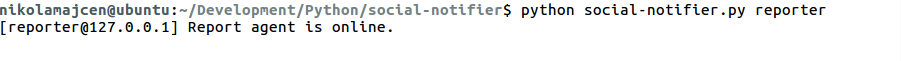
\includegraphics[width=\linewidth, frame]{01-starting-reporter}
	\caption{Pokretanje agenta izvjestitelja}
\end{figure}

Kada je agent izvjestitelj aktivan, moguće je pokrenuti i ostale agente. Ovdje ću za početak prikazati rad Twitter agenta i to tako da traži nove statuse sa određenih hashtag-om. Za pokretanje Twitter agenta koristi se sjedeći način pokretanja koji se može vidjeti na slici 4.2. zajedno sa načinom rada agenta. Važno je reći da su u ovom slučaju uneseni samo potrebni parametri odnosno argumenti, a svi ostali argumenti odnosno parametri programa su zadani u slučaju ako nisu uneseni od strane korisnika.

\begin{figure}[h]
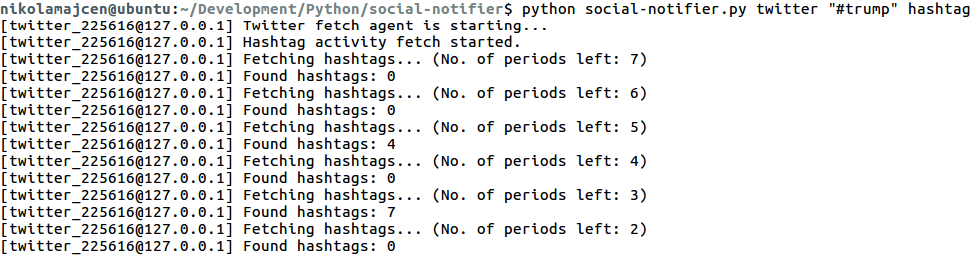
\includegraphics[width=\linewidth, frame]{02-starting-twitter-hashtag}
		\caption{Pokretanje Twitter agenta za hashtag pretragu}
\end{figure}

Kako agent, u ovom slučaju Twitter agent, dohvaća nove statuse sa zadanih hashtag-om, on ispisuje koliko je statusa dohvatio u pojedinom periodu te odbrojava broj preostalih perioda. U svakom od tih perioda šalje agentu izvjestitelju u realnom vremenu podatke o dohvaćenim statusima ukoliko ih ima. Agent izvjestitelj te podatke dohvaća, ispisuje i sprema u rječnik.

\begin{figure}[h]
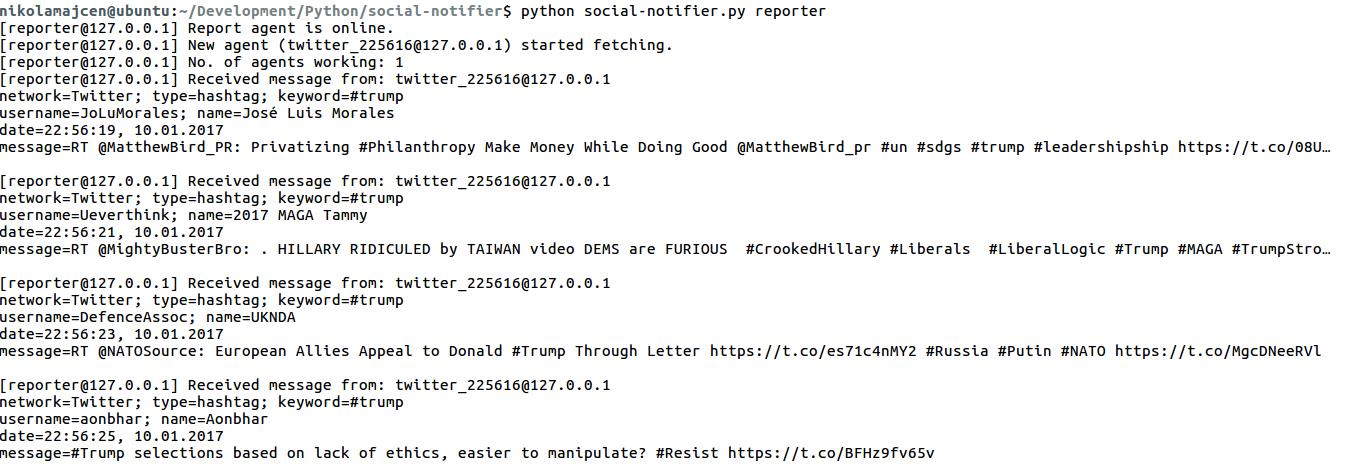
\includegraphics[width=\linewidth, frame]{03-getting-messages-from-twitter-agent}
	\caption{Dobivanje poruka od Twitter agenta}
\end{figure}

Nakon što Twitter agent dohvati podatke određen broj puta, Twitter agent šalje nakon toga zahtjev za konačnim izvještajem o svim dohvaćenim podacima, a rezultat toga može se vidjeti na slici 4.4. 

Sve do ovog koraka, Twitter agent ne zna koje je sve podatke dohvatio, već su svi podaci pohranjeni kod agenta izvjestitelja. Upravo zato potrebno je da se na kraju svakog rada pojedinog agenta zatraži izvještaj sa svim dohvaćenim podacima koje se nalaze kod agenta izvjestitelja.

\begin{figure}[h]
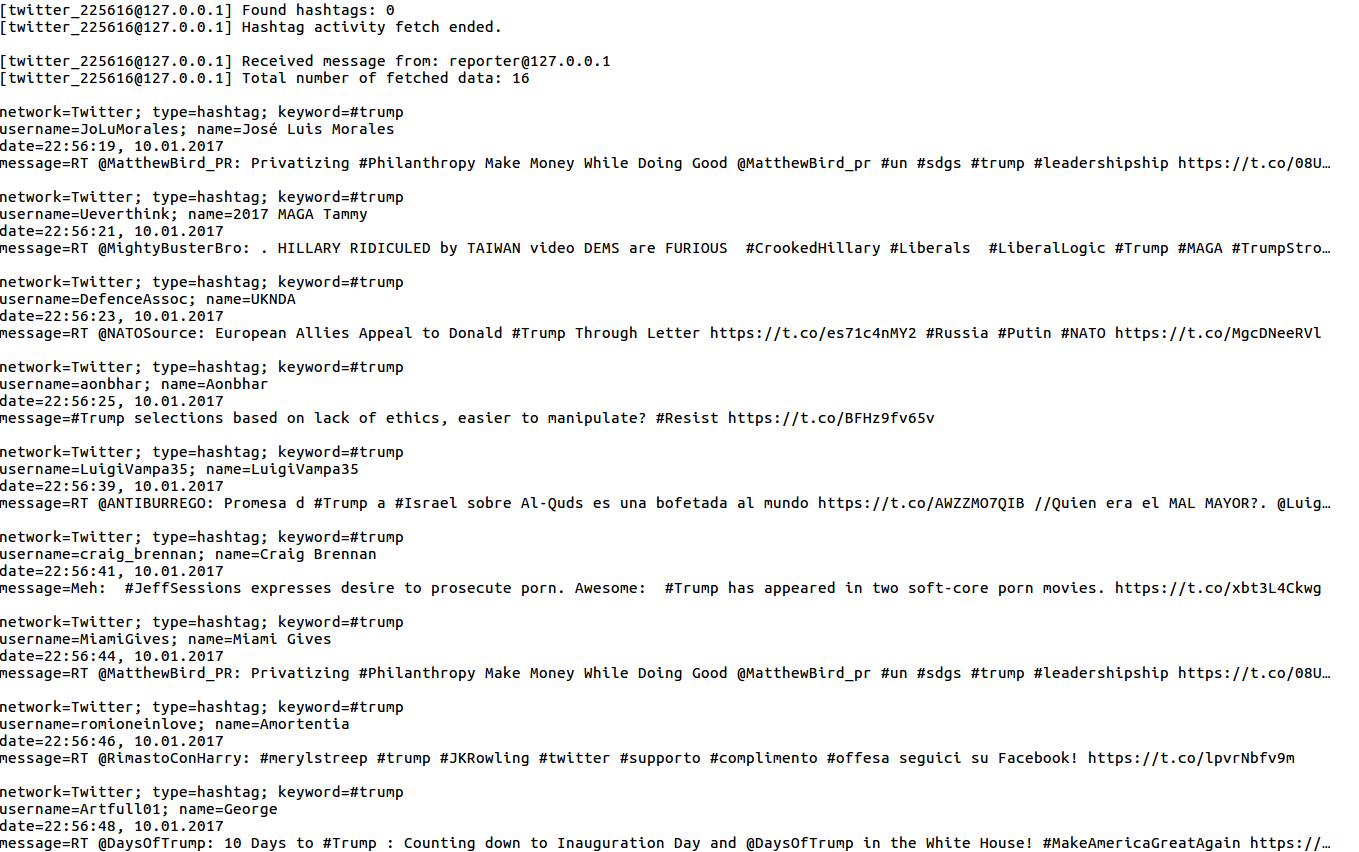
\includegraphics[width=\linewidth, frame]{04-getting-report}
	\caption{Dobivanje izvještaja od strane agenta izvjestitelja}
\end{figure}

Kada je Twitter agent dobio konačni izvještaj, on završava sa radom. Toga je svjestan i agent izvjestitelj, te on prikazuje novo stanje broja aktivnih agenata svaki puta kada pošalje izvještaj pojedinom agenta. Razlog tome je što svaki agent završava s radom kad dobije izvještaj o dohvaćanju podataka pa se na temelju toga može vidjeti koliko je još aktivnih agenata. 

Naravno, novi agenti se registriraju na početku rada svakog agenta, tako da se i u tom slučaju ispisuju podaci o aktivnim agentima. Primjer praćenja broja agenata može se vidjeti na slici 4.5.

\begin{figure}[h]
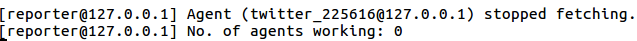
\includegraphics[width=\linewidth, frame]{05-agent-stopped}
	\caption{Ažuriranje broja aktivnih agenata}
\end{figure}

Drugi način rada Twitter agenta je dohvaćanje statusa pojedinog korisnika, tako da se umjesto tipa \texttt{hashtag} unese \texttt{tweet}. Također, potrebno je umjesto ključne riječi ovaj put unijeti korisničko ime korisnika čije statuse se želi pratiti.

\begin{figure}[h]
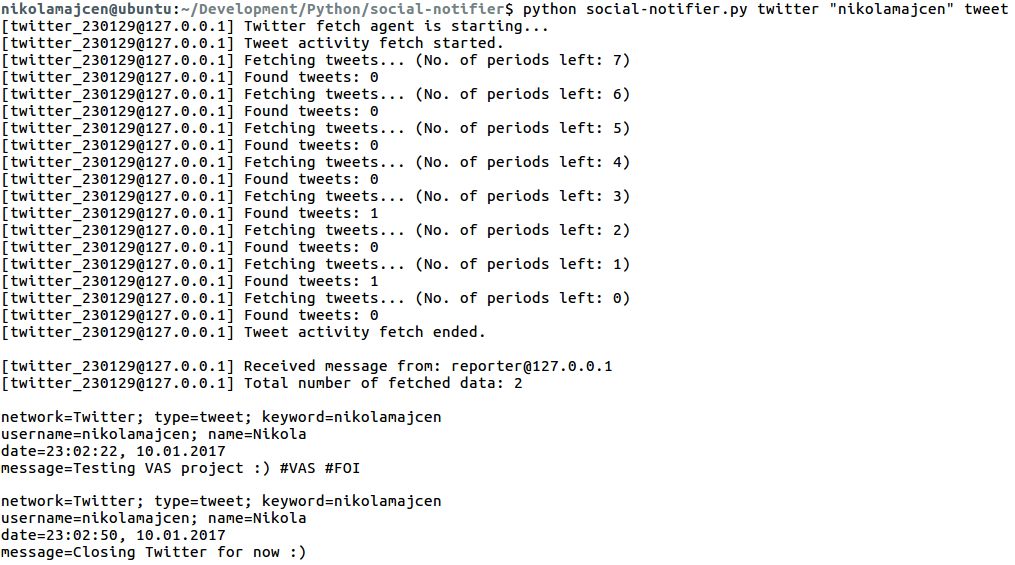
\includegraphics[width=\linewidth, frame]{06-twitter-tweet-fetch}
	\caption{Pokretanje Twitter agenta za dohvaćanjem statusa korisnika}
\end{figure}

Na slici 4.6 se može vidjeti rad tj. pokretanje Twitter agenta uz način rada \texttt{tweet} koji definira dohvaćanje novih statusa određenog korisnika. 

Agent u određenom broju perioda dohvaća statuse navedenog korisnika, te pronađene statuse šalje agentu izvjestitelju. Agent u ovom slučaju ne zna za podatke koje je dohvatio, nego iste direktno šalje agentu izvjestitelju kod kojeg su pohranjeni svi dohvaćeni podaci. Iz tog razloga, kada dohvaćanje podataka završi, Twitter agent od agenta izvjestitelja dobiva izvještaj sa svim dohvaćenim statusima navedenog korisnika.

Kako to izgleda kod agenta izvjestitelja, moguće je vidjeti slici 4.7. Moguće je vidjeti početak rada agenta, što zapravo predstavlja registraciju Twitter agenta kod agenta izvjestitelja čime se povećav broj trenutnih aktivnih agenata. U svakom od perioda šalju se dohvaćeni podaci agentu izvjestitelju koji te podatke ispisuje te ih sprema u rječnik. Podaci su kod agenta izvjestitelja tako dugo dok Twitter agent dohvaća podatke.

Kada Twitter agent završi s dohvaćanjem, zatraži od agenta izvjestitelja da mu pošalje izvještaj sa svim podacima. Upravo ovdje se vidi da je agent završio s radom te se nakon slanja izvještaja broj aktivnih agenata smanjuje za jedan.

Ovime je završena demonstracija Twitter agenta, gdje su prikazana dva načina rada i to; dohvaćanje statusa na temelju hashtag-a od strane svih korisnika društvene mreže te dohvaćanje statusa pojedinog korisnika na temelju unesenog korisničkog imena od strane korisnika.

Moguće je uz navedene načine pokretanja programa još i promijeniti vrijeme trajanja dohvaćanja podataka, vrijeme trajanja jedne periode pa sve do promjene naziva konfiguracijske datoteke ili datoteke s podacima za spajanje na društvenu mrežu. 

\begin{figure}[h]
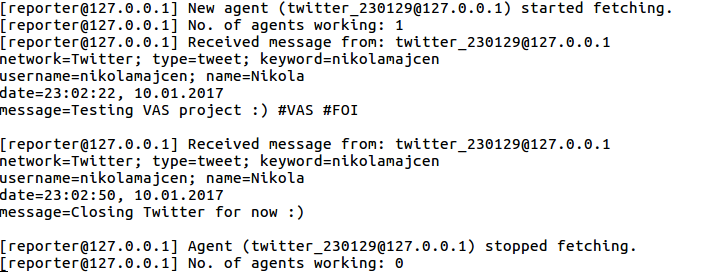
\includegraphics[width=\linewidth, frame]{07-reporter-getting-all-tweets-data}
	\caption{Dohvaćanje statusa od strane agenta izvjestitelja}
\end{figure}

Sljedeći agent je Facebook agent, koji dohvaća statuse ili slike sa profila korisnika. Važno je napomenuti da u ovom slučaju to radi sa profilima koji su javno dostupni, a ne i sa privatnim profilima korisnika na društvenoj mreži Facebook.

Kod pokretanja ovog agenta iskoristio sam mogućnost promjene opcionalnih parametara, tako da je promijenjeno ukupno vrijeme dohvaćanja odnosno argument \texttt{time} i vrijeme trajanja jedne periode odnosno argument \texttt{period}. Uz navedene argumente, obavezno je i unijeti korisničko ime profila koji se želi pratiti.

Agent radi na isti način kao i Twitter agent, tako da dohvaća podatke u zadanih periodima, te ih u svakom periodu šalje agentu izvjestitelju ukoliko su podaci dohvaćeni. 

Na kraju rada agenta, šalje se zahtjev za izvještajem, a agent izvjestitelj šalje izvještaj s podacima ukoliko su podaci dohvaćeni. U ovom slučaju nisu dohvaćeni nikakvi podaci u smislu statusa ili slika na navedenom profilu, tako da izvješće ne sadrži nikakve podatke, već se u izvješću nalazi samo broj dohvaćenih podataka, što je u ovom slučaju nula (0).

\begin{figure}[h]
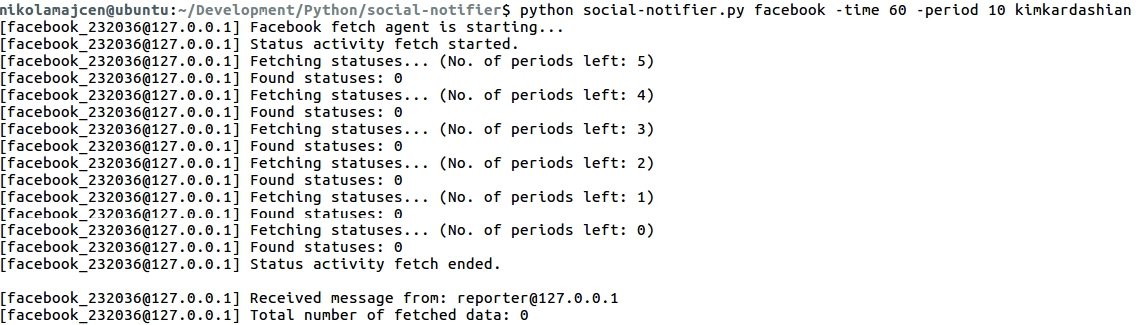
\includegraphics[width=\linewidth, frame]{08-facebook-fetch}
	\caption{Pokretanje Facebook agenta}
\end{figure}

Vrijedi još prikazati rad agenta izvjestitelja sa više agenata, odnosno prikazati kako se prikazuje rad s više agenata i njihovih promjena u dohvaćanju podataka. Ovo je vrlo važna odlika rada agenta, jer je vrlo važno omogućiti da više agenata mogu istovremeno raditi sa agentom izvjestiteljem. 

Na slici 4.9 može se vidjeti primjer rada agenta izvjestitelja sa više agenata koji dohvaćaju podatke s društvenih mreža.

\begin{figure}[h]
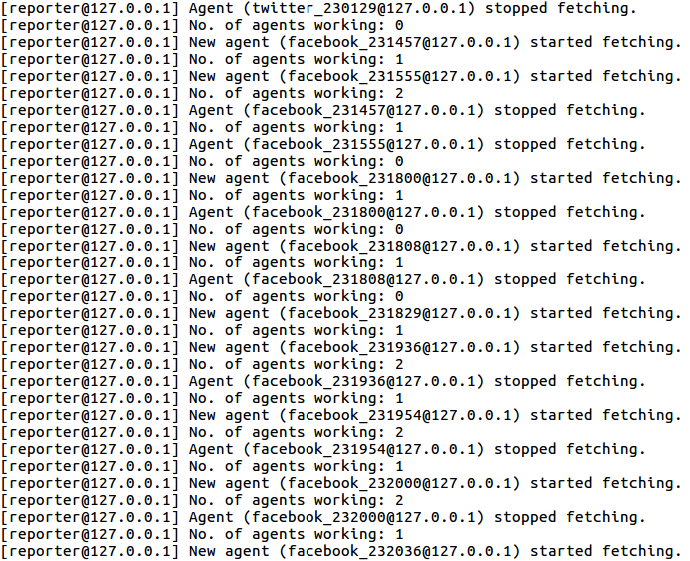
\includegraphics[width=\linewidth, frame]{09-reporter-multiconnect}
	\caption{Prikaz rada agenta izvjestitelja s više agenata}
\end{figure}

% Zaključak

\chapter{Zaključak}

% Literatura

\addcontentsline{toc}{chapter}{Bibliografija}
\bibliography{foi.bib}
\end{document}
